\tikzsetexternalprefix{tikz/}	% set subfolder
\tikzsetnextfilename{LVTcurves}
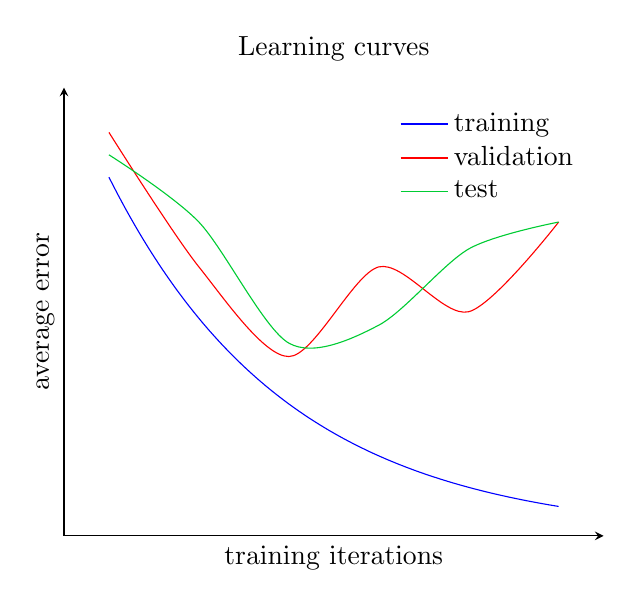
\begin{tikzpicture}[baseline]
	\begin{axis}[
			title ={Learning curves},
			xlabel={training iterations},
			ylabel={average error},
			axis x line=bottom,
			axis y line=left,
			domain=0:5,
			xmin=-0.5, xmax=5.5,
			ymin=0,	ymax=1,
			ticks=none,
			legend style={draw=none},
			legend pos= north east,
			legend entries={training,validation,test},
			legend cell align=left,
		]

		\addplot [blue, samples=101, smooth]	{.8*exp(-0.5*x)};
		
		\addplot [red, smooth] coordinates {
			(0.0,0.9)
			(1.0,0.6)
			(2.0,0.4)
			(3.0,0.6)
			(4.0,0.5)
			(5.0,0.7)
		};
		
		\addplot [green!80!blue, smooth] coordinates {
			(0.0,0.85)
			(1.0,0.7)
			(2.0,0.43)
			(3.0,0.47)
			(4.0,0.64)
			(5.0,0.7)
		};
		
%		\addplot [black, only marks, mark=o] coordinates {(2.0,0.4)}
		
	\end{axis}
\end{tikzpicture}